% Nome do capítulo
\chapter{Experimentos}
% Label para referenciar
\label{cap:5}
% Diminuir espaçamento entre título e texto
\vspace{-1.9cm}

\section{SSD}
\label{secao:5:1}

A primeira implementação consiste em adaptar a \ac{DenseNet} 121 para realizar as tarefas de localização e classificação. Nesse estágio foi feita uma pequena alteração com relação aos modelos propostos por \citeonline{wei-2015} e por \citeonline{cheng-2017}. Enquanto que \citeonline{wei-2015} usou imagens de tamanho $300 \times 300$ e \citeonline{cheng-2017} usou imagens de tamanho $321\times 321$, foi usado nesse trabalho imagens de $311 \times 311$.

O motivo é que, embora a \ac{DenseNet} possua as mesmas características de \textit{downsample} (por meio de convolução ou \textit{pooling}) que a \ac{ResNet}, a implementação da \ac{SSD} por \citeonline{cheng-2017} usa \textit{padding} válido para todas as camadas de \textit{downsample}. Isso faz com que, caso o tamanho de saída da camada de \textit{downsample} não seja inteiro, uma parte seja cortada, podendo causar perda de informação. Sendo assim, foi feita a opção por uma imagem com tamanho menor e o uso de \textit{padding} equivalente, de forma a evitar o corte.

Além dessas modificações, é necessário mudar algumas coisas na arquitetura da rede \ac{DenseNet}121. A primeira delas é que a SSD utiliza ramificações de diferentes níveis para fazer as predições de forma mais precisa. Sendo assim, a primeira alteração é que no segundo bloco de transição é criada uma ramificação fazendo regularização L2. Além disso, a camada de \textit{pooling} do último bloco de transição é substituída por um bloco $3\times3$ com strides igual a 1. No final da rede as camadas de \textit{pooling} global e softmax são removidas e essa saída é a segunda ramificação da \ac{SSD}. Depois disso, são adicionados mais dois blocos com camadas de convolução, uma $1\times1$ seguida de um $3\times3$ com \textit{stride} 2. Por fim, mais dois blocos, com as mesmas camadas, porém, as camadas $3\times3$ com \textit{stride} igual a 1.

\subsection{Treinamento}
\label{secao:5:1:1}

A rede foi inicializada com os pesos da \ac{DenseNet}121 treinada na ImageNet, e as camadas adicionais foram inicializadas com o método \textit{He normal} proposto por \citeonline{he-2015}. O algoritmo de treinamento selecionado foi o Adam, proposto por \citeonline{kingma-2014} com os seguintes hiperparâmetros:

\begin{itemize}
	\item $\alpha = 5\times10^{-5}$;
	\item $\beta_1 = 0,9$;
	\item $\beta_2 = 0,999$;
	\item $\epsilon = 1\times10^{-8}$.
\end{itemize}

Além disso, o treinamento ocorreu em um total de 400 épocas, cada época com 1000 iterações e cada iteração com um lote de processamento de 12 imagens. Após 200 épocas de treinamento, a taxa de aprendizado caiu para $5\times10^{-6}$ e após mais 100 épocas, caiu para $5\times10^{-7}$. As bases de dados usadas para os testes foram a \ac{PASCAL VOC} 2007 e 2012. Para treinamento foram usadas as imagens do conjunto de treino e validação de ambas as bases, e para validação dos testes foi utilizada a base de testes de 2007. Os testes serão feitos na base de 2012.

\subsection{Avaliação Qualitativa}
\label{secao:5:1:2}

Depois do treinamento, foram feitos alguns experimentos com imagens aleatórias do conjunto separado para validação para avaliar os resultados obtidos pelo método. Embora o método consiga fazer a detecção e a classificação dos objetos, foram percebidas algumas dificuldades.

\begin{figure}[H]
	% Alterar espaçamentos antes e depois do caption
	\setlength{\abovecaptionskip}{0pt}
	\setlength{\belowcaptionskip}{0pt}
	% Caption
	\caption[Resultado dos testes 1]{Resultado dos testes 1}
	\centering
	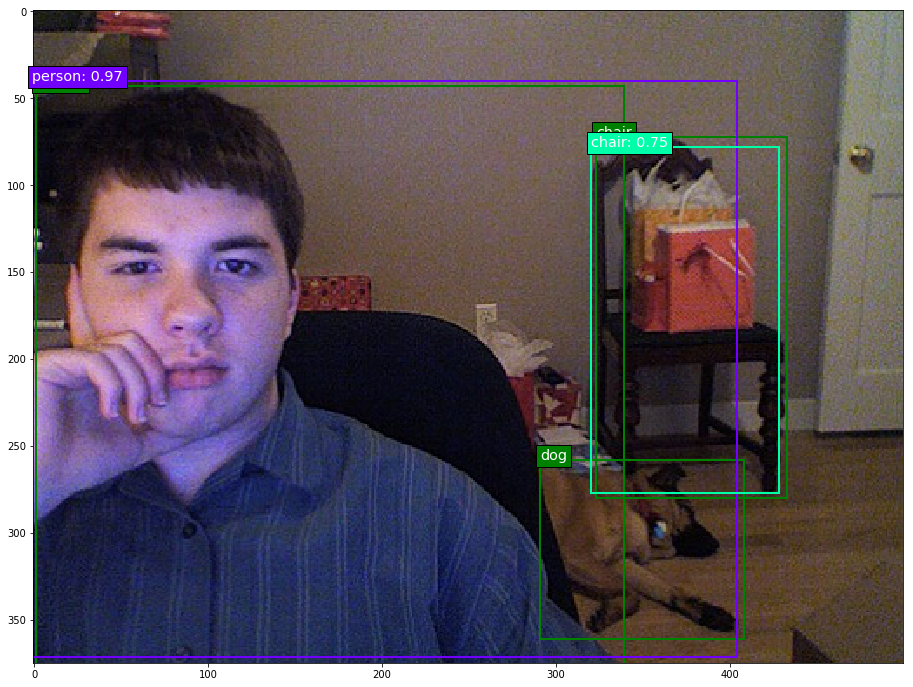
\includegraphics[width=.6\textwidth]{imagem/test_image_5.png}
	% Caption centralizada
	\captionsetup{justification=centering}
	\captionfont{\small{\textbf{\\Fonte: Elaborado pelo autor.}}}	
	\label{fig:teste_1}
\end{figure}

Na Figura \ref{fig:teste_1} o modelo detectou a pessoa sentada na cadeira e a cadeira no fundo, porém não detectou o cão deitado no chão. Isso pode refletir um pouco de dificuldade em perceber objetos menores ou que não estejam tão centralizados. Além disso, Embora a pessoa sentada esteja bem nítida na imagem, o modelo não conseguiu ter 100\% de confiança que era uma pessoa.

\begin{figure}[H]
	% Alterar espaçamentos antes e depois do caption
	\setlength{\abovecaptionskip}{0pt}
	\setlength{\belowcaptionskip}{0pt}
	% Caption
	\caption[Resultado dos testes 2]{Resultado dos testes 2}
	\centering
	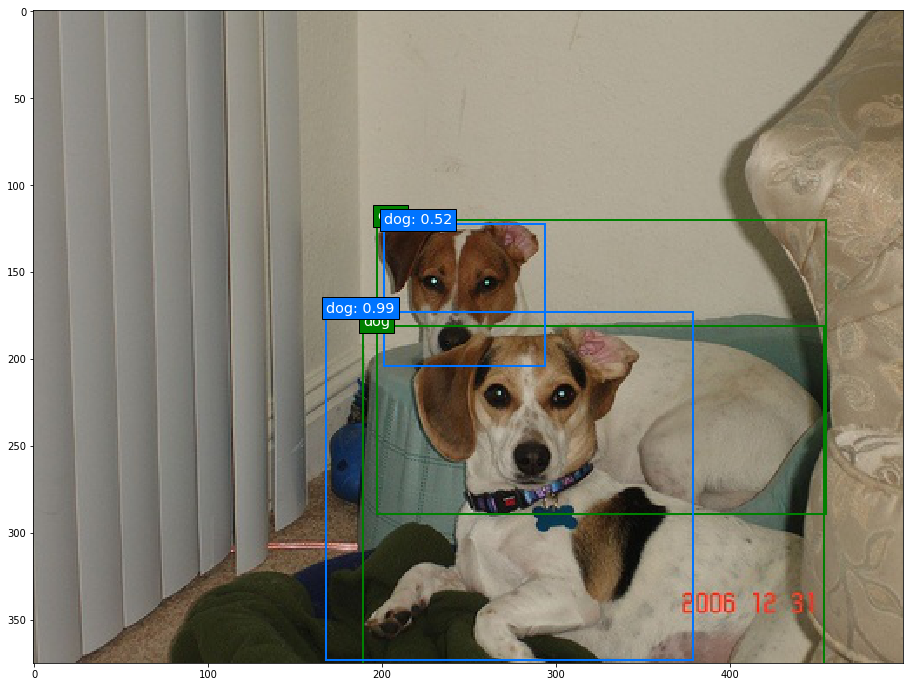
\includegraphics[width=.6\textwidth]{imagem/test_image_3.png}
	% Caption centralizada
	\captionsetup{justification=centering}
	\captionfont{\small{\textbf{\\Fonte: Elaborado pelo autor.}}}	
	\label{fig:teste_2}
\end{figure}

Na Figura \ref{fig:teste_2} percebemos mais uma vez o problema da confiança baixa. Além disso, a \textit{bounding box} do cão de trás esta pegando apenas a cabeça, sendo que outras partes do corpo dele estão expostas (ainda que sobrepostas parcialmente).


\begin{figure}[H]
	% Alterar espaçamentos antes e depois do caption
	\setlength{\abovecaptionskip}{0pt}
	\setlength{\belowcaptionskip}{0pt}
	% Caption
	\caption[Resultado dos testes 3]{Resultado dos testes 3}
	\centering
	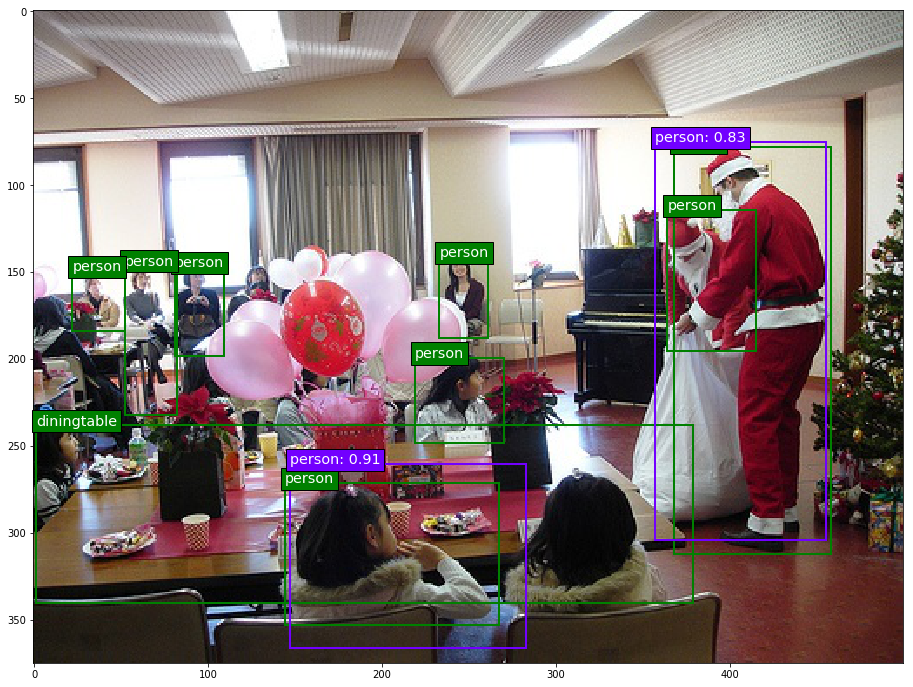
\includegraphics[width=.6\textwidth]{imagem/test_image_1.png}
	% Caption centralizada
	\captionsetup{justification=centering}
	\captionfont{\small{\textbf{\\Fonte: Elaborado pelo autor.}}}	
	\label{fig:teste_3}
\end{figure}

Na Figura \ref{fig:teste_3}, mostra mais uma vez uma nítida dificuldade do modelo em perceber objetos mais distantes. A imagem possui 9 objetos delimitados no \textit{ground-truth} e o modelo conseguiu detectar apenas 2. Ele não consegue perceber nem a mesa de jantar e nem as pessoas mais ao fundo. Além disso, as duas pessoas que estão em pé no canto direito da Figura foram percebidas como apenas uma pelo modelo.


\begin{figure}[H]
	% Alterar espaçamentos antes e depois do caption
	\setlength{\abovecaptionskip}{0pt}
	\setlength{\belowcaptionskip}{0pt}
	% Caption
	\caption[Resultado dos testes 4]{Resultado dos testes 4}
	\centering
	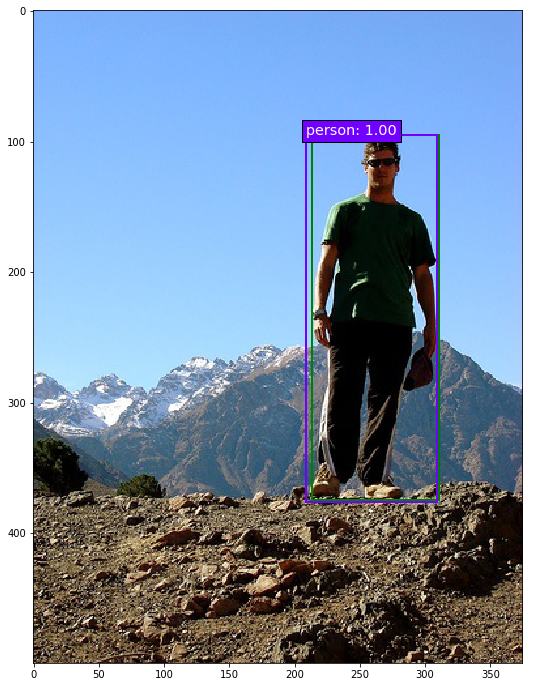
\includegraphics[width=.6\textwidth]{imagem/test_image_2.png}
	% Caption centralizada
	\captionsetup{justification=centering}
	\captionfont{\small{\textbf{\\Fonte: Elaborado pelo autor.}}}	
	\label{fig:teste_4}
\end{figure}

A Figura \ref{fig:teste_4} é bem simples e o único objeto presente está bem nítido, então o modelo consegue percebê-lo com a confiança de 100\%.

\begin{figure}[H]
	% Alterar espaçamentos antes e depois do caption
	\setlength{\abovecaptionskip}{0pt}
	\setlength{\belowcaptionskip}{0pt}
	% Caption
	\caption[Resultado dos testes 5]{Resultado dos testes 5}
	\centering
	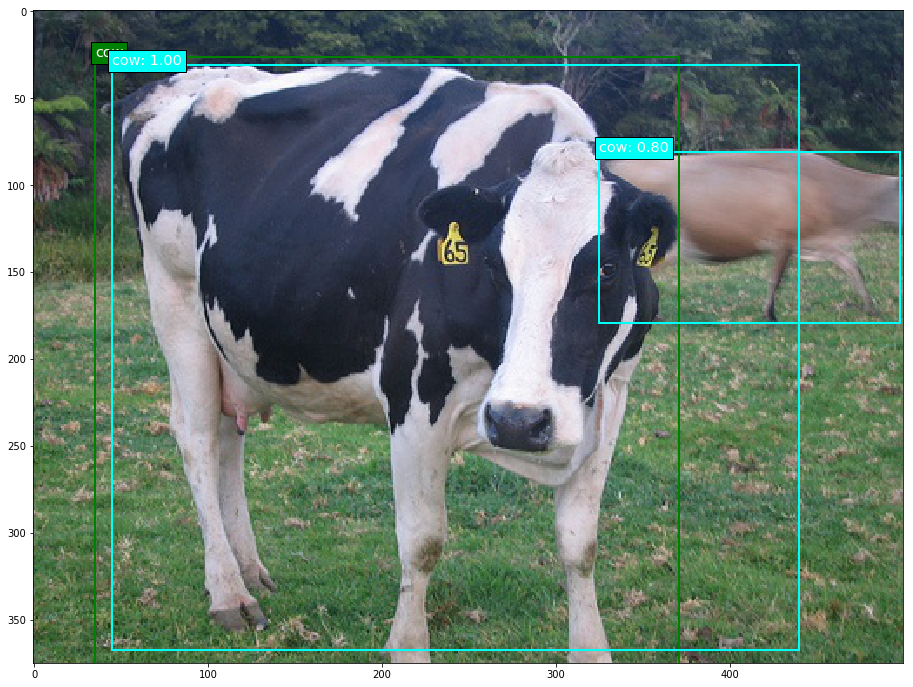
\includegraphics[width=.6\textwidth]{imagem/test_image_4.png}
	% Caption centralizada
	\captionsetup{justification=centering}
	\captionfont{\small{\textbf{\\Fonte: Elaborado pelo autor.}}}	
	\label{fig:teste_5}
\end{figure}

Já a Figura \ref{fig:teste_5} mostra um fenômeno diferente: além de detectar o único objeto presente no \textit{ground-truth} com a confiança alta, ele também detecta uma outra instância do mesmo objeto ao fundo. Isso significa que embora o modelo tenha um pouco de dificuldade com objetos que não estão em destaque, essa dificuldade não é tão crítica e existe uma certa robustês.

\subsection{Avaliação Quantitativa}
\label{secao:5:1:3}

Depois dos experimentos, foram feitos os testes para avaliar de forma numérica os resultados do modelo e comparar com o estado da arte. O resultado final apontou um \ac{mAP} de 72,6\%. 

  \begin{table}[H]
    \centering
    \footnotesize
% Alterar espaçamentos antes e depois do caption
    \setlength{\abovecaptionskip}{0pt}
    \setlength{\belowcaptionskip}{0pt}
% Caption
    \caption[Resultados SSD]{Comparação SSD300, SSD321 e SSD311}
    \label{tab:resultados}
% Conteúdo da tabela
    \begin{tabular}{c|c|c|c}
	Objeto &	SSD311(nosso) & SSD300 & SSD321 \\ 
	\hline 
 	Avião 			& 80,8\%	& 79,5\% 	& 76,3\% \\ 
	Bicicleta 		& 82,3\%	& 83,9\% 	& 84,6\%  \\ 
	Pássaro 		& 66,3\%	& 76\%  	& 79,3\%  \\
	Barco 			& 61,3\%	& 69,6\% 	& 64,6\%  \\ 
	Garrafa 		& 31,2\%	& 57,5\%  	& 47,2\%  \\ 
	Ônibus 			& 82,8\%	& 87\%	 	& 85,4\%  \\
	Carro 			& 86\%		& 85,7\%  	& 84\%  \\ 
	Gato 			& 85,8\%	& 88,1\%  	& 88,8\%  \\
	Cadeira 		& 52,9\%	& 60,3\%  	& 60,1\%  \\ 
	Vaca 			& 75\% 		& 81,5\% 	& 82,6\%  \\
	Mesa de Jantar 	& 72,4\% 	& 77\%  	& 76,9\%  \\ 
	Cão 			& 77,4\% 	& 86,1\% 	& 86,7\%  \\
	Cavalo 			& 86,2\% 	& 87,5\% 	& 87,2\%  \\ 
	Motocicleta 	& 86,3\% 	& 84\%  	& 85,4\%  \\
	Pessoa 			& 77,4\% 	& 79,4\%  	& 79,1\%  \\ 
	Vaso de planta 	& 42,6\% 	& 52,3\%  	& 50,8\%  \\
	Ovelha 			& 69,9\%	& 77,9\%  	& 77,2\%  \\
	Sofá 			& 77,2\% 	& 79,5\%  	& 82,6\%  \\
	Trem 			& 84,3\% 	& 87,6\%  	& 87,3\%  \\
	Monitor/TV 		& 73\% 		& 76,8\%  	& 76,6\%  \\ 
	Total 			& 72,6\% 	& 77,5\%  	& 77,1\%  \\
    \end{tabular}
% Fonte
    \\
    \captionfont{\small{\textbf{\\Fonte: Elaborado pelo autor.}}}
  \end{table}

% Fazer analise comparativa com os resultados.
Com base na Tabela \ref{tab:resultados} podemos ver que os resultados estão um pouco abaixo dos obtidos por \citeonline{wei-2015} e \citeonline{cheng-2017}. Apesar disso, pode-se observar que o modelo se saiu muito bem em algumas classes como Avião, Carro, Motocicleta, Cavalo e bicicleta, chegando a ter resultados melhores que os outros modelos em algumas delas.

A principal dificuldade está nos objetos mais difíceis, onde o modelo não conseguiu se ajustar bem, e acabou apresentando resultados muito inferiores aos obtidos pelos outros métodos. Entre essas classes, podemos destacar o vaso de planta, a cadeira, e a Garrafa. Algumas dessas classes o modelo perde por uma discrepância de mais de 10 pontos percentuais.

A diferença nos resultados se deve a alguns fatores. Entre eles podemos citar o tamanho do lote de treinamento. Enquanto o nosso modelo foi treinado com 12 imagens por lote, os modelos de \citeonline{wei-2015} e \citeonline{cheng-2017} foram treinados usando um lote de 32 imagens. 

Além disso, devido ao número menor no lote de treinamento, foi necessário aumentar o número de épocas e iterações para garantir a convergência. O aumento de iterações com lotes menores pode causar um \textit{Overfitting} que é quando o modelo aprende os dados específicos ao invés de aprender a generalizar com base nos dados.

% O resultado evidencia algumas dificuldades que o modelo apresentou conforme visto na seção \ref{secao:5:1:2} e não está no mesmo nível que os resultados obtidos por \citeonline{wei-2015} e \citeonline{cheng-2017}.

% Esse problema pode ser justificado por dois fatores principais. Por limitações computacionais, só foi possível fazer o treinamento com 12 imagens por iteração, enquanto que os modelos de \citeonline{wei-2015} e \citeonline{cheng-2017} treinaram com 32 imagens por iteração. Pelo fato do número de imagens por iteração ser menor, foi necessário treinar por mais iterações o que pode acarretar em um segundo problema: \textit{overfitting}, que é quando o modelo começa a aprender os dados específicos ao invés de aprender a fazer a classificação de forma mais generalista.